

\chapter{VsnLib}                %crea il capitolo
%%%%%%%%%%%%%%%%%%%%%%%%%%%%%%%%%%%%%%%%%imposta l'intestazione di pagina
\lhead[\fancyplain{}{\bfseries\thepage}]{\fancyplain{}{\bfseries\rightmark}}
Strato di compatibilit\`a tra pacchetti netlink e stack di rete virtuali.

\section{Il Progetto}                 %crea la sezione
Gli stack analizzati in precedenza offrono a grandi linee la stessa tipologia di servizio seppur ognuna con le proprie caratteristice.\\
Nessuno dei progetti ha per\`o tenuto in considerazione l'idea di utilizzare un'interfaccia di configurazione che fosse standard e pertanto \`e necessario usare le funzioni specifiche per ognuno di questi progetti, costringendo il programmatore a cambiare modalit\`a di interazione da stack a stack.\\
Il progetto di creare questa libreria nasce proprio da questa esigenza, ovvero cercare di uniformare le interfacce di comunicazione in modo tale che l'utente non sia costretto ad adattarsi ogni qual volta decida di cambiare stack.\\


\section{Sviluppo}
Risulta subito chiaro dalla successiva immagine che il progetto si compone di un core che comprende una parte client ed una server.\\

\begin{figure}[h]                       %crea l'ambiente figura; [h] sta
                                        %   per here, cio� la figura va qui
\begin{center}                          %centra nel mezzo della pagina
                                        %   la figura
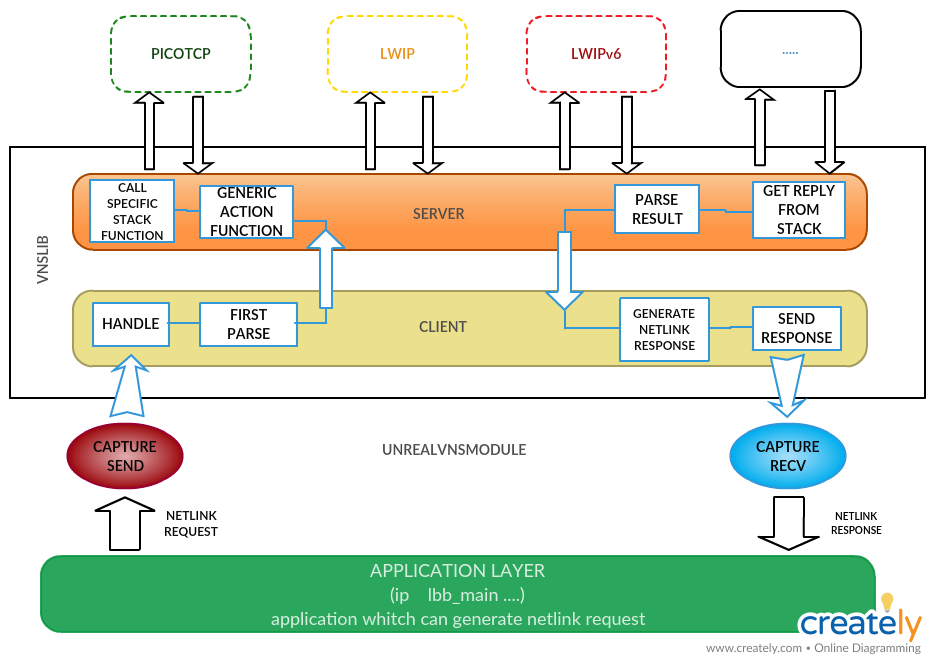
\includegraphics[width=15cm]{vnslib_scheme}%inserisce una figura larga 5cm
                                        %se si vuole usare va scommentata
%
%%%%%%%%%%%%%%%%%%%%%%%%%%%%%%%%%%%%%%%%%inserisce la legenda ed etichetta
                                        %   la figura con \label{fig:prima}
\caption[mappa concettuale libreria]{mappa concettuale libreria}\label{fig:map}
\end{center}
\end{figure}
\`E facile immaginare che la suddivisione riguardi l'interazione della libreria con l'utente.
\begin{description}                     %crea un elenco descrittivo
  \item[Client-side:] risiedono le funzioni che catturano i pacchetti netlink e che quindi permettono le configurazioni attraverso l'interfaccia netlink. In questa fase ci si occupa di fare parsing del pacchetto per costruire una struttura contenente i dati significativi.
  \item[Server-side:] back end della libreria, qui vengono gestiti i dati passati dal client per poi chiamare le specifiche funzioni approntate per configurare lo stack in uso.
\end{description}

\section{Moduli}
\section{Il Futuro}
%%%%%%%%%%%%%%%%%%%%%%%%%%%%%%%%%%%%%%%%%non numera l'ultima pagina sinistra
\clearpage{\pagestyle{empty}\cleardoublepage} 
